%%%%%%%%%%%%%%%%%%%%%%%%%%%%%%%%%%%%%%%%%
% Short Sectioned Assignment
% LaTeX Template
% Version 1.0 (5/5/12)
%
% This template has been downloaded from:
% http://www.LaTeXTemplates.com
%
% Original author:
% Frits Wenneker (http://www.howtotex.com)
%
% License:
% CC BY-NC-SA 3.0 (http://creativecommons.org/licenses/by-nc-sa/3.0/)
%
%%%%%%%%%%%%%%%%%%%%%%%%%%%%%%%%%%%%%%%%%

%----------------------------------------------------------------------------------------
%	PACKAGES AND OTHER DOCUMENT CONFIGURATIONS
%----------------------------------------------------------------------------------------

\documentclass[paper=a4, fontsize=11pt]{scrartcl} % A4 paper and 11pt font size

\usepackage[T1]{fontenc} % Use 8-bit encoding that has 256 glyphs
\usepackage{fourier} % Use the Adobe Utopia font for the document - comment this line to return to the LaTeX default
\usepackage[english]{babel} % English language/hyphenation
\usepackage{amsmath,amsfonts,amsthm} % Math packages

\usepackage{graphicx}

\usepackage{sectsty} % Allows customizing section commands
\allsectionsfont{\centering \normalfont\scshape} % Make all sections centered, the default font and small caps

\usepackage[procnames]{listings}

\usepackage{fancyhdr} % Custom headers and footers
\pagestyle{fancyplain} % Makes all pages in the document conform to the custom headers and footers
\fancyhead{} % No page header - if you want one, create it in the same way as the footers below
\fancyfoot[L]{} % Empty left footer
\fancyfoot[C]{} % Empty center footer
\fancyfoot[R]{\thepage} % Page numbering for right footer
\renewcommand{\headrulewidth}{0pt} % Remove header underlines
\renewcommand{\footrulewidth}{0pt} % Remove footer underlines
\setlength{\headheight}{13.6pt} % Customize the height of the header

\numberwithin{equation}{section} % Number equations within sections (i.e. 1.1, 1.2, 2.1, 2.2 instead of 1, 2, 3, 4)
\numberwithin{figure}{section} % Number figures within sections (i.e. 1.1, 1.2, 2.1, 2.2 instead of 1, 2, 3, 4)
\numberwithin{table}{section} % Number tables within sections (i.e. 1.1, 1.2, 2.1, 2.2 instead of 1, 2, 3, 4)

\setlength\parindent{0pt} % Removes all indentation from paragraphs - comment this line for an assignment with lots of text

%----------------------------------------------------------------------------------------
%	TITLE SECTION
%----------------------------------------------------------------------------------------

\newcommand{\horrule}[1]{\rule{\linewidth}{#1}} % Create horizontal rule command with 1 argument of height

\title{	
\normalfont \normalsize 
\textsc{BRSU} \\ [25pt] % Your university, school and/or department name(s)
\horrule{0.5pt} \\[0.4cm] % Thin top horizontal rule
\huge Neural Networks\\Assignment 5 \\ % The assignment title
\horrule{2pt} \\[0.5cm] % Thick bottom horizontal rule
}

\author{Bastian Lang} % Your name

\date{\normalsize\today} % Today's date or a custom date

\begin{document}

\maketitle % Print the title

\newpage

This report contains the summary, ex3.1 and ex3.2 without any programming/plotting.

\section{Summary}
Please see figures \ref{fig1} - \ref{fig6}.
\begin{figure}[ht]
	\centering
  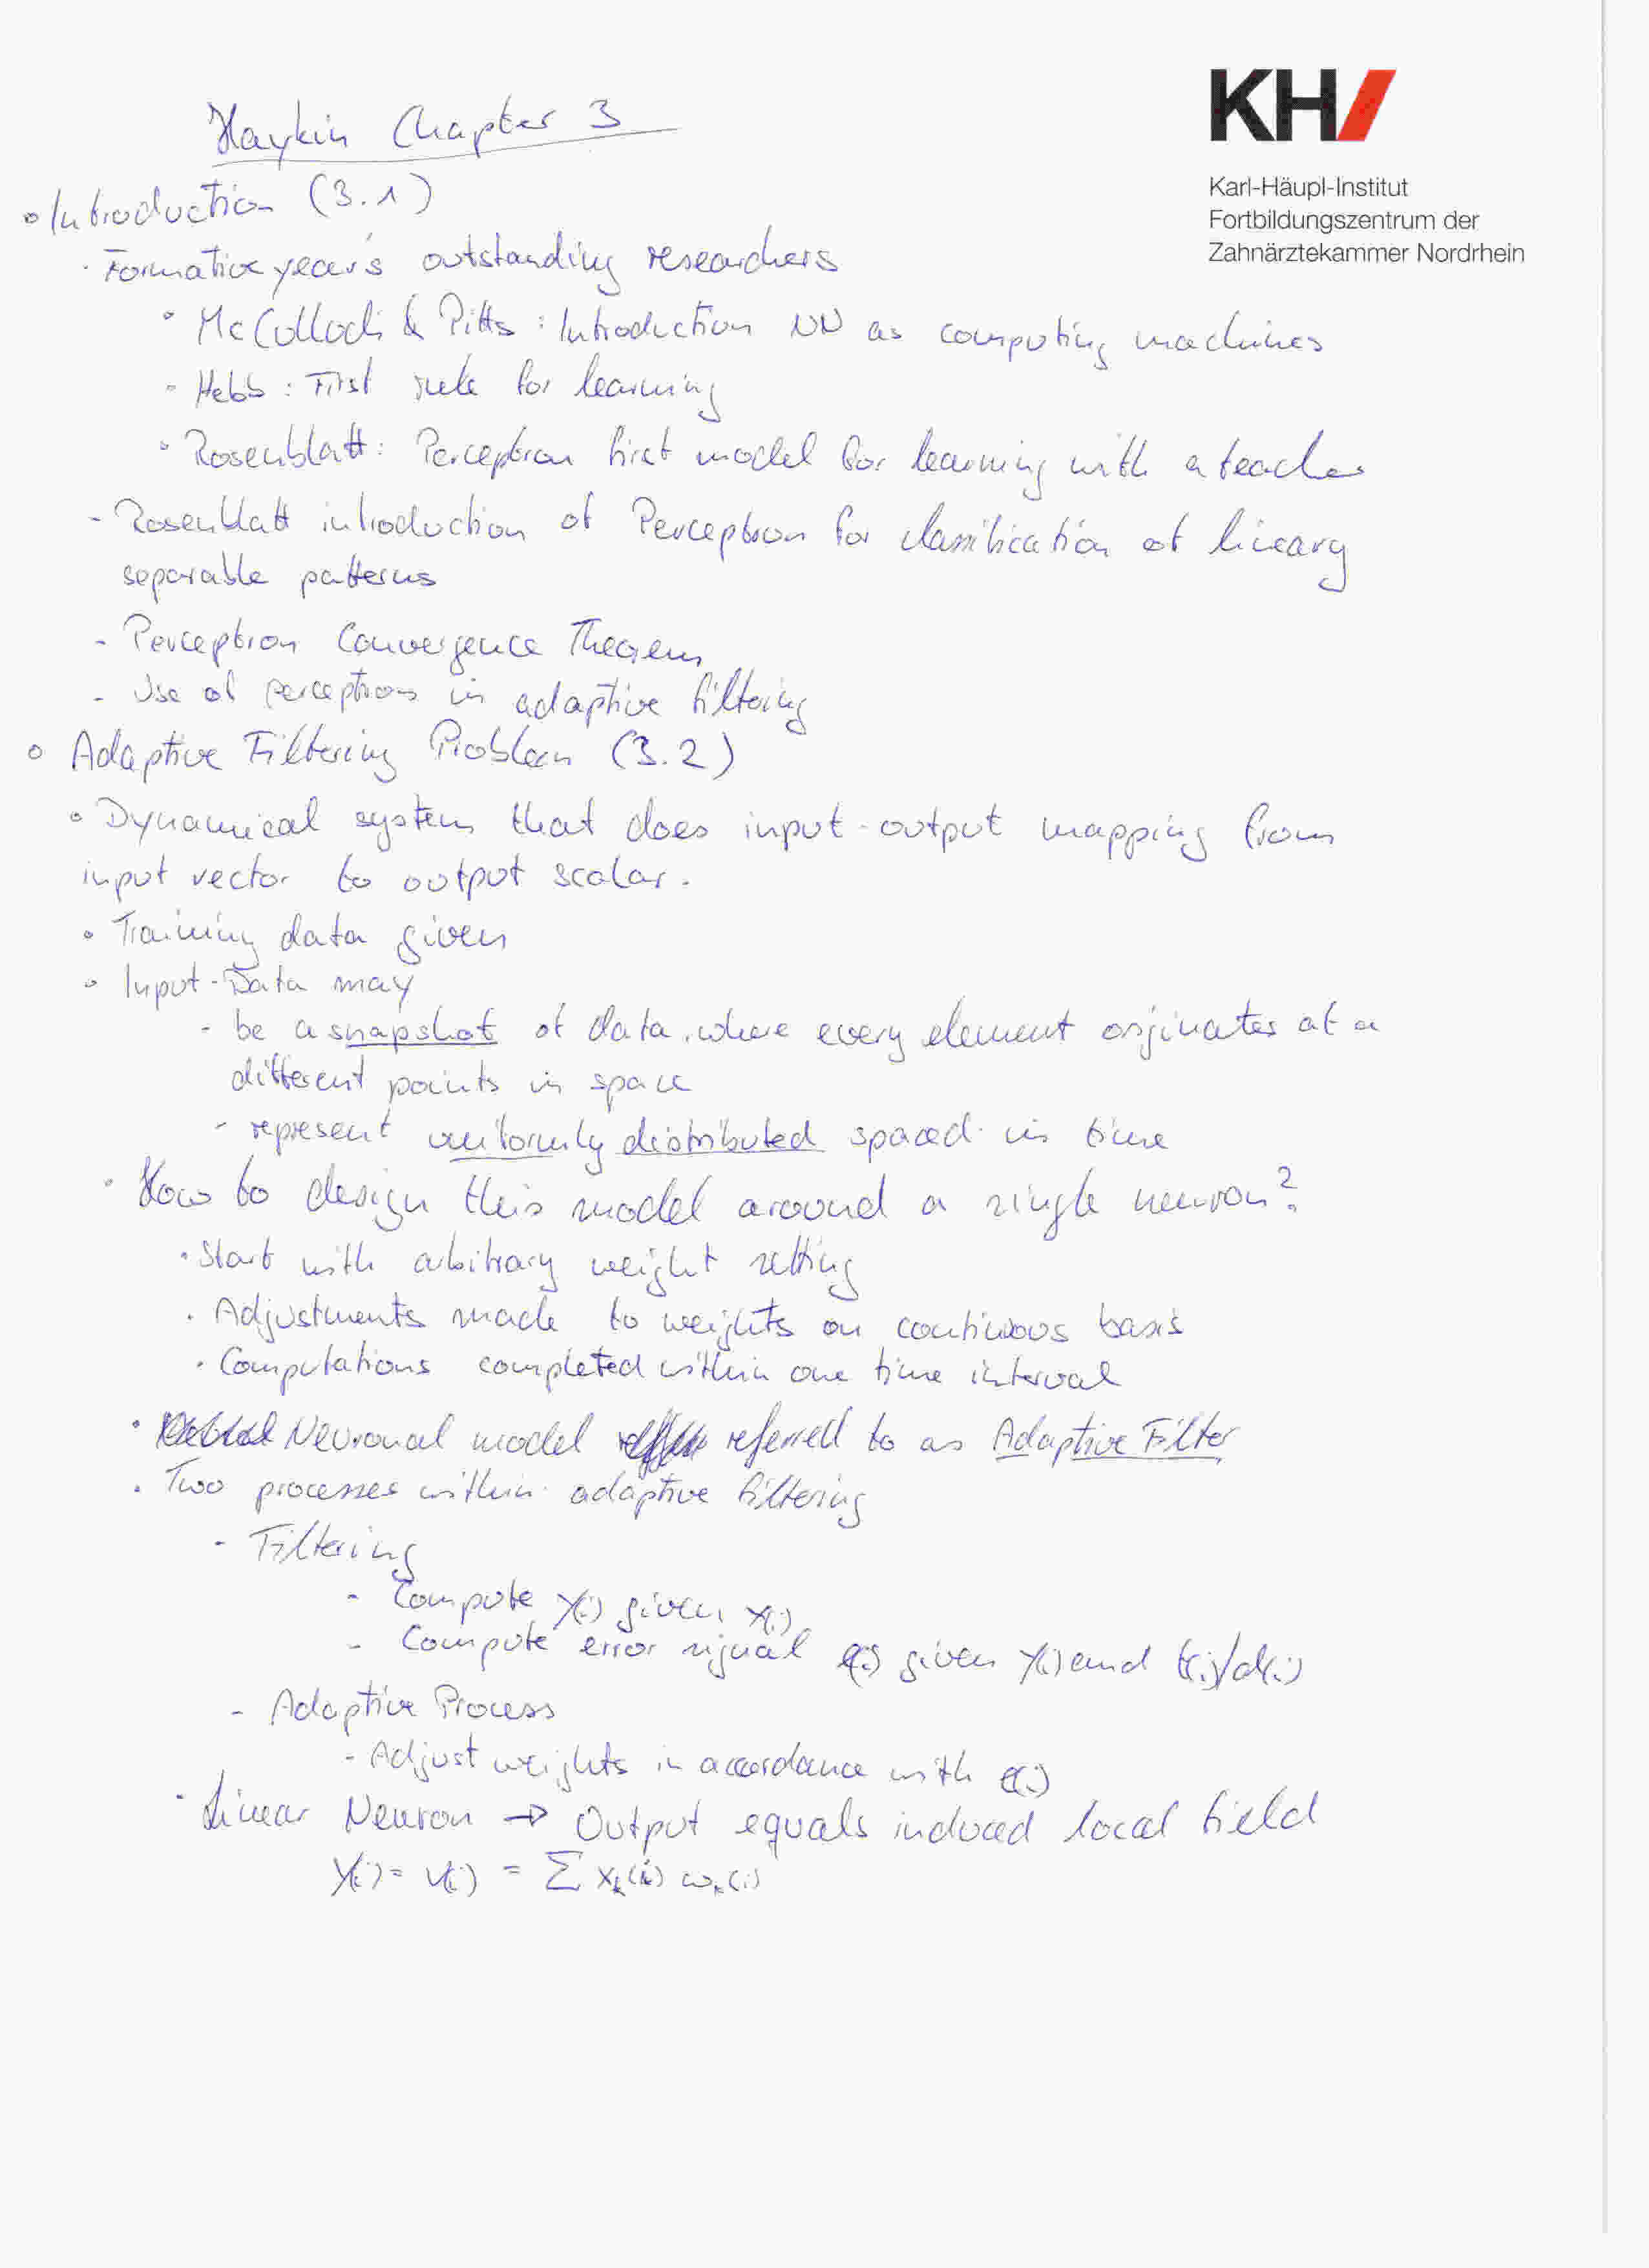
\includegraphics[width=0.7\textheight]{04.jpg}
	\caption{summary 1}
	\label{fig1}
\end{figure}

\begin{figure}[ht]
	\centering
  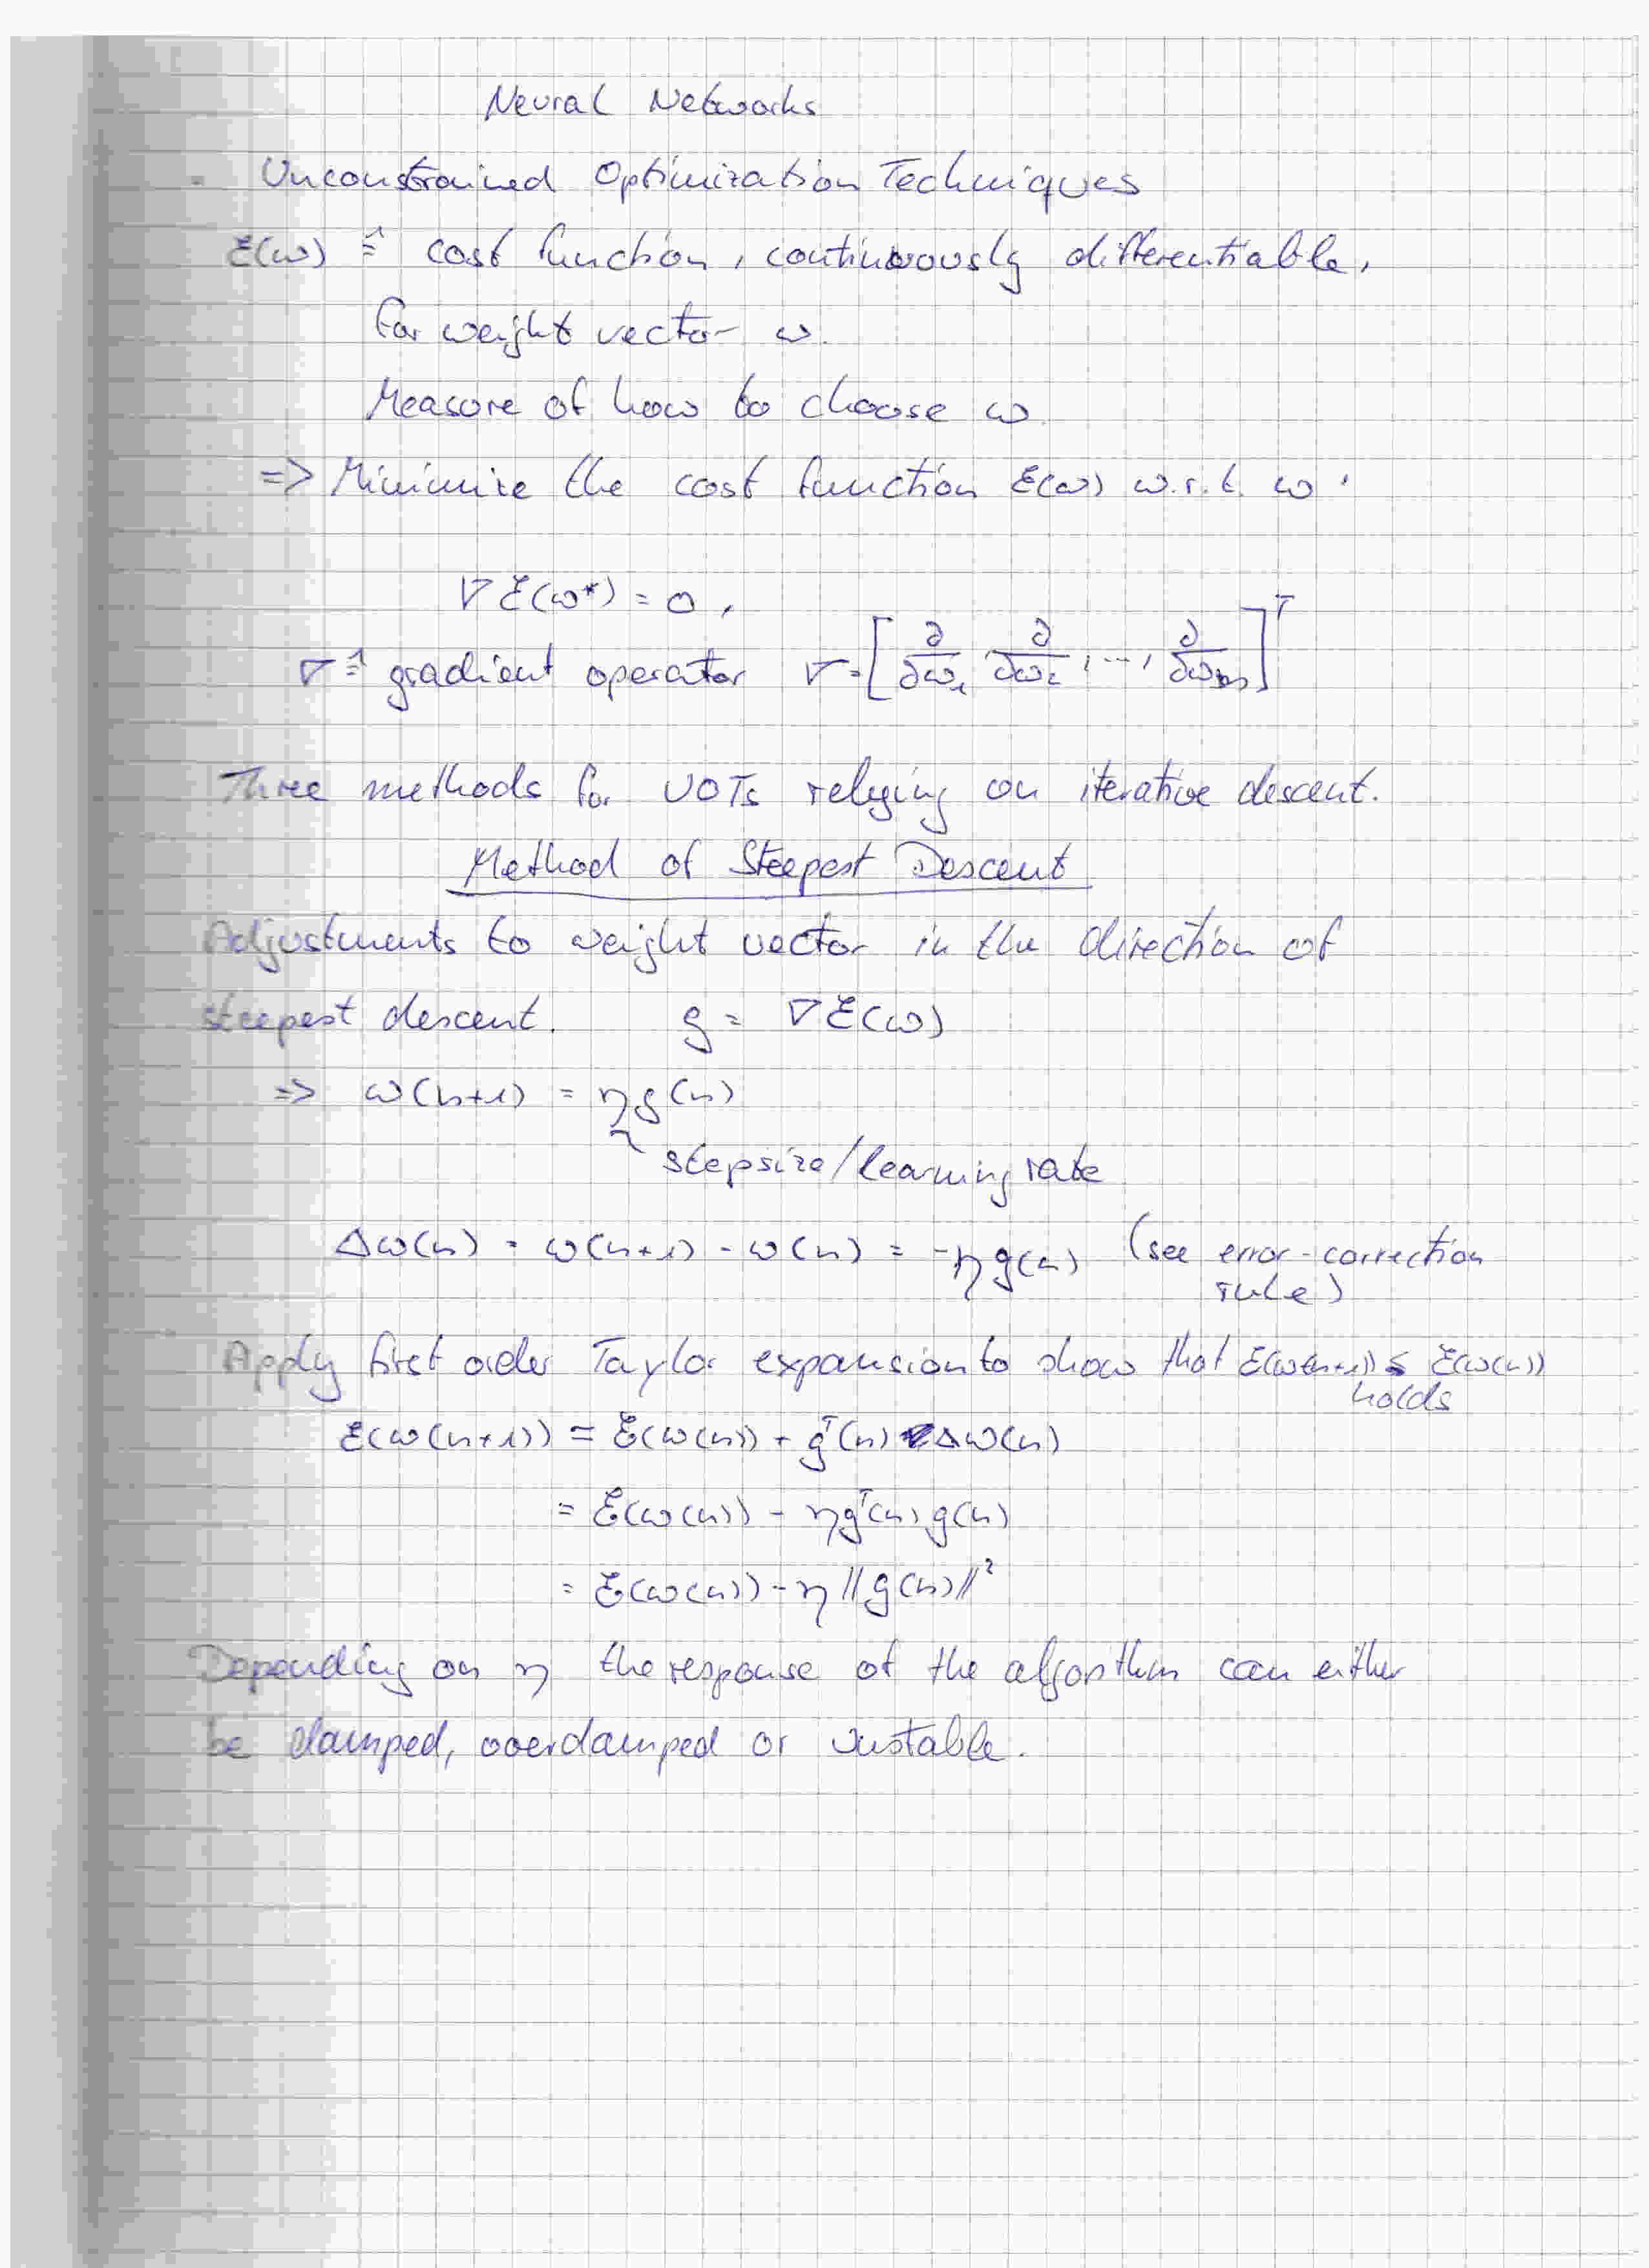
\includegraphics[width=0.7\textheight]{05.jpg}
	\caption{summary 2}
	\label{fig2}
\end{figure}

\begin{figure}[ht]
	\centering
  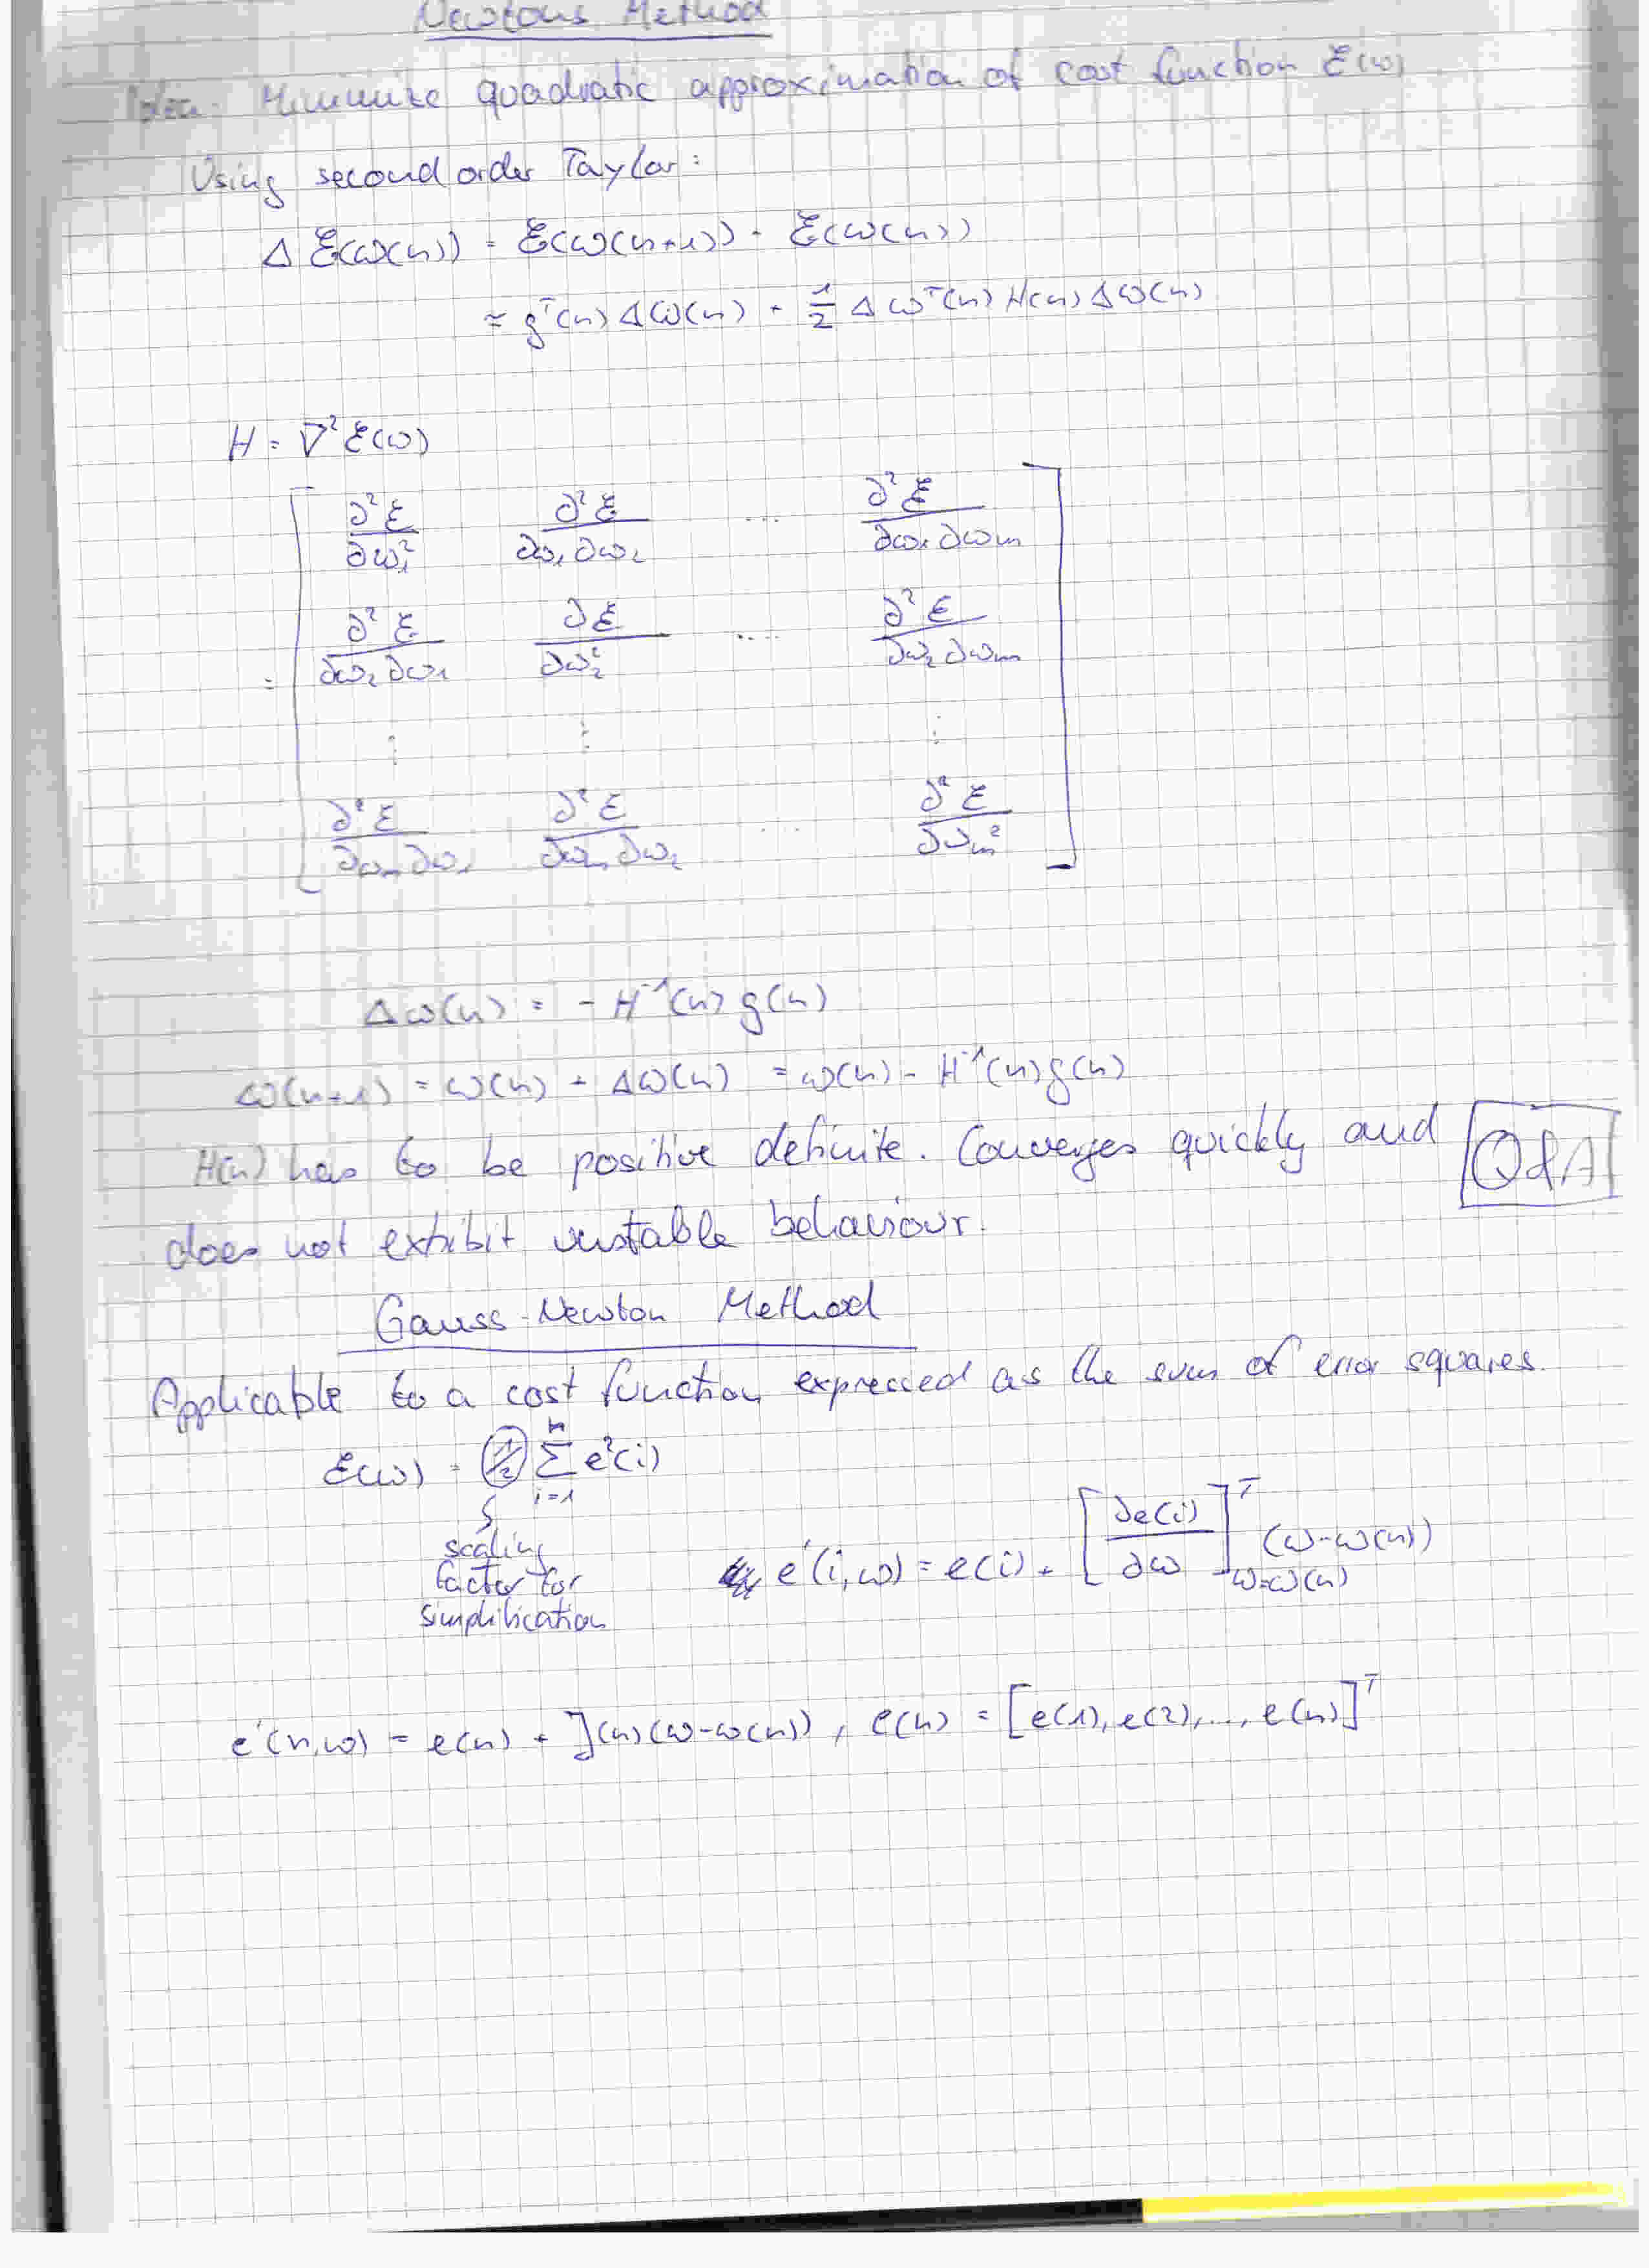
\includegraphics[width=0.7\textheight]{06.jpg}
	\caption{summary 3}
	\label{fig3}
\end{figure}

\begin{figure}[ht]
	\centering
  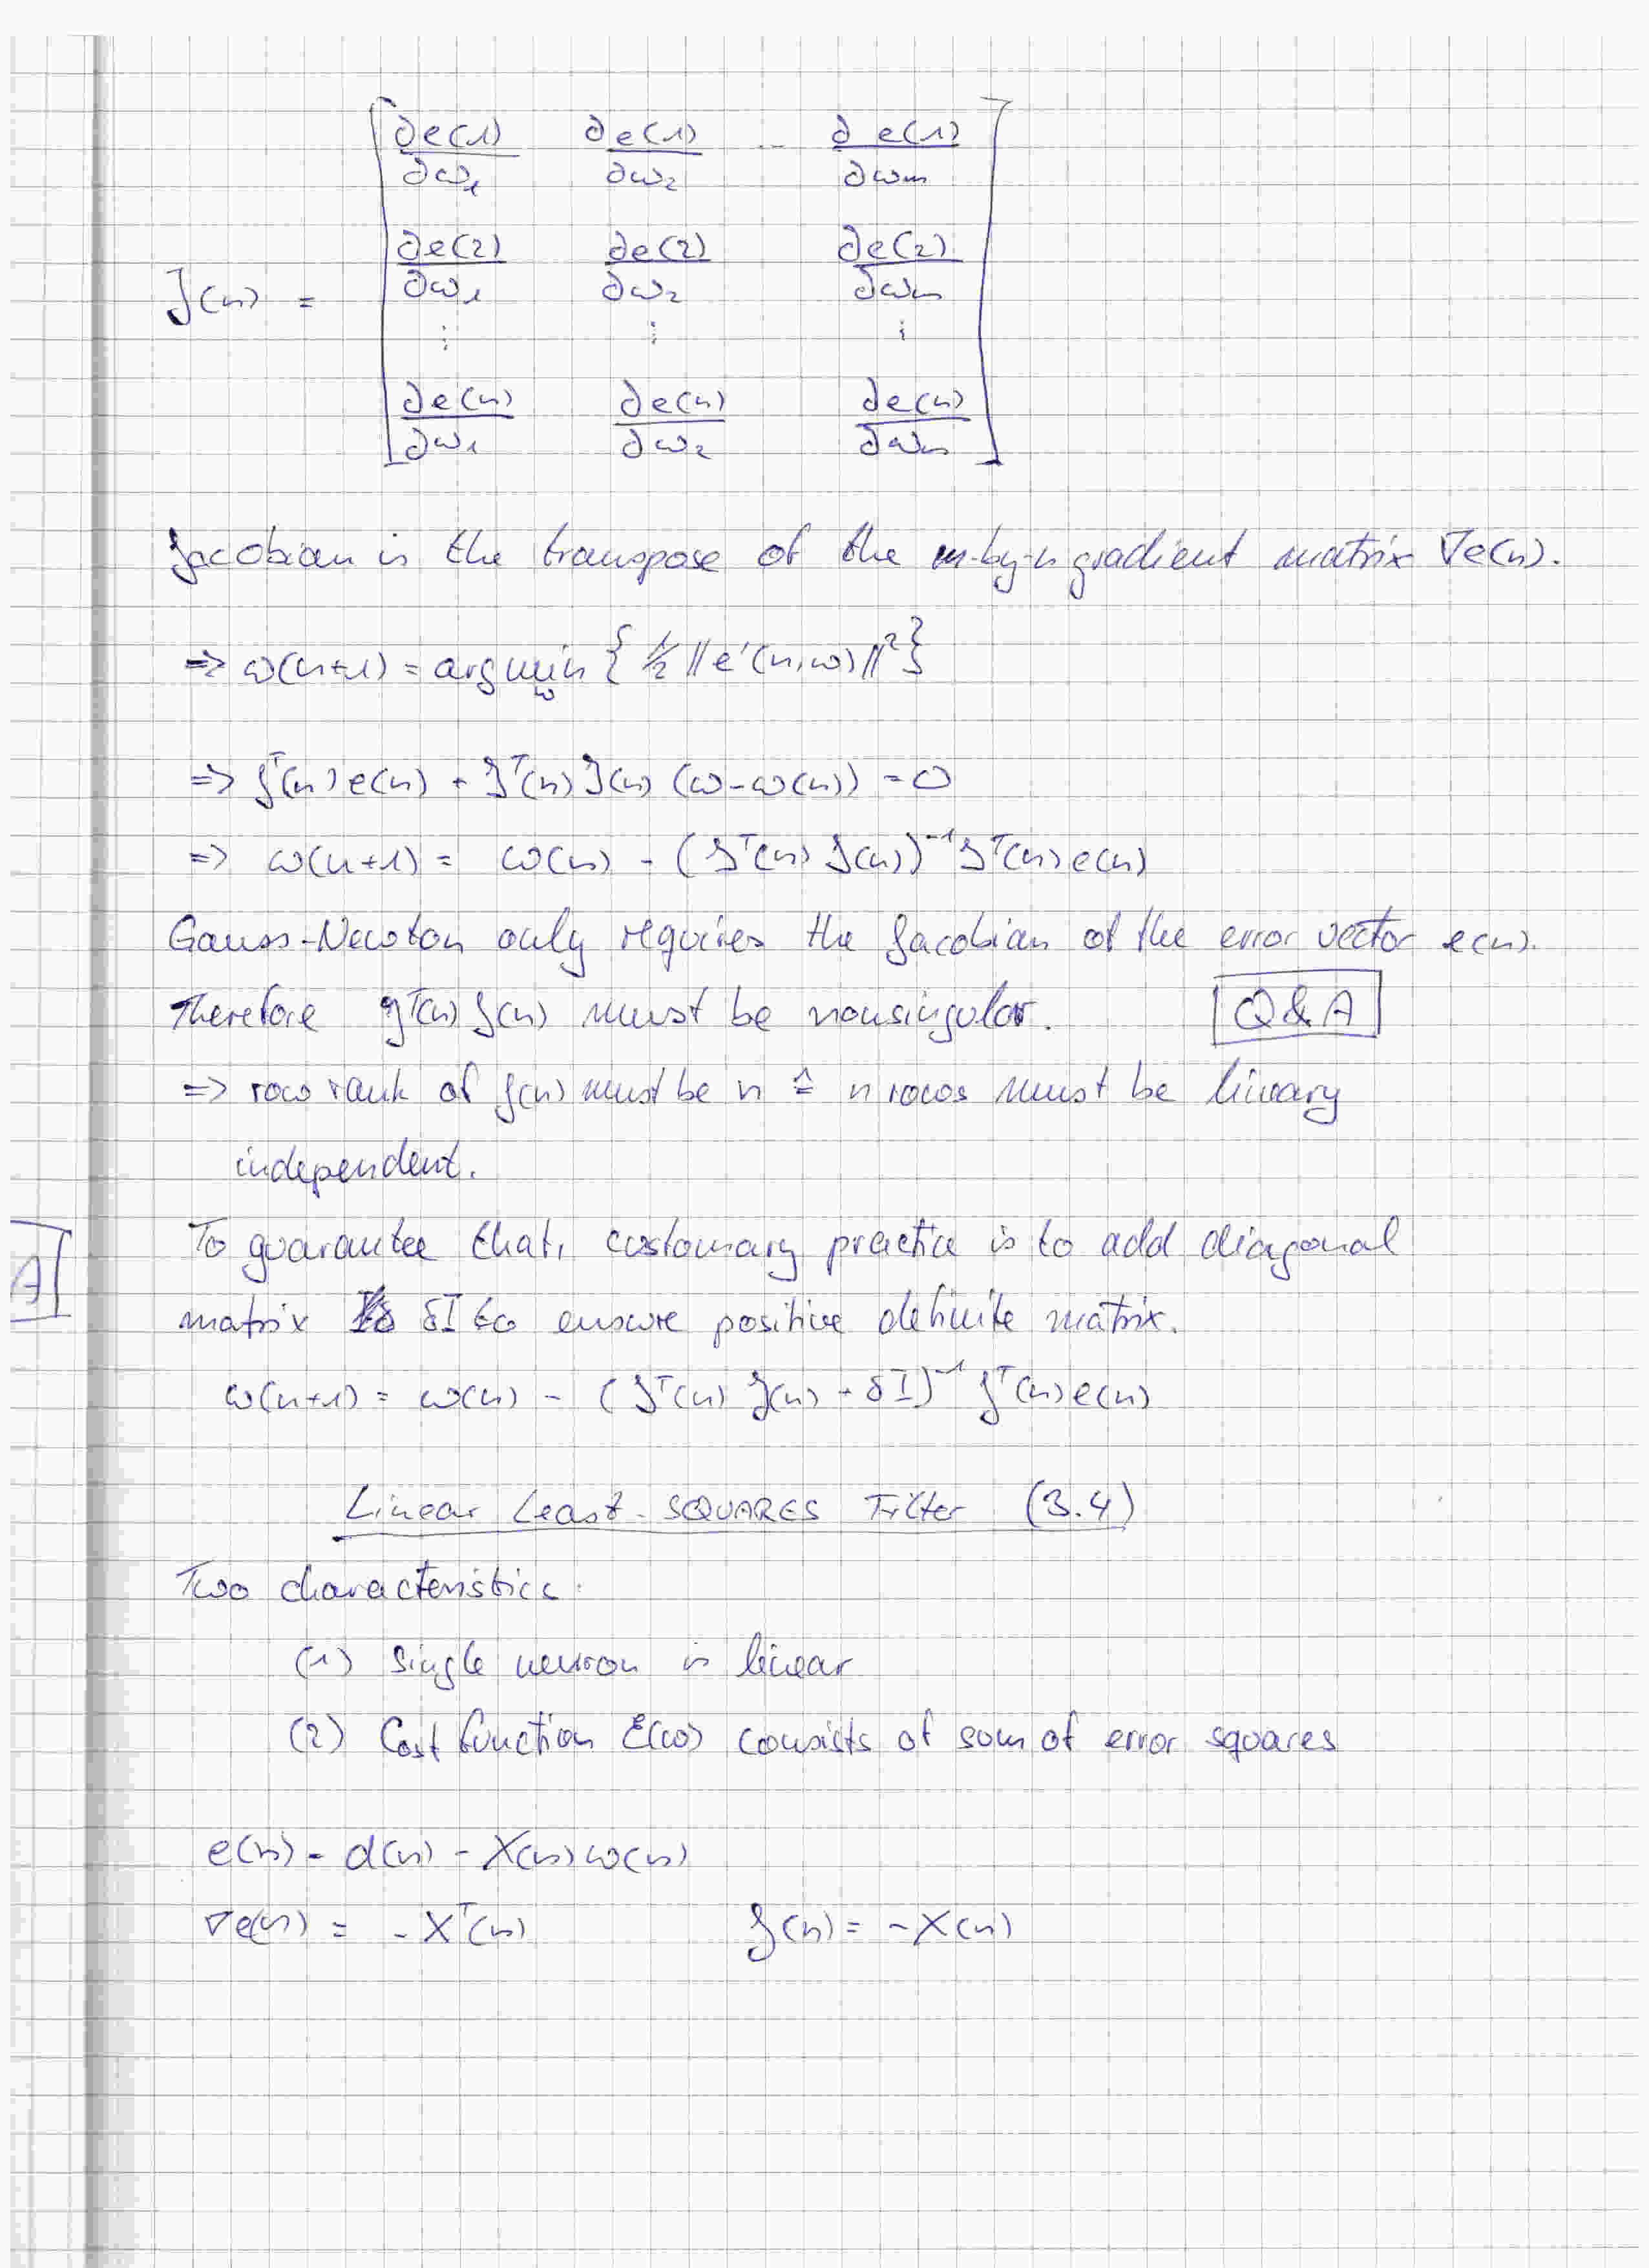
\includegraphics[width=0.7\textheight]{07.jpg}
	\caption{summary 4}
	\label{fig4}
\end{figure}

\begin{figure}[ht]
	\centering
  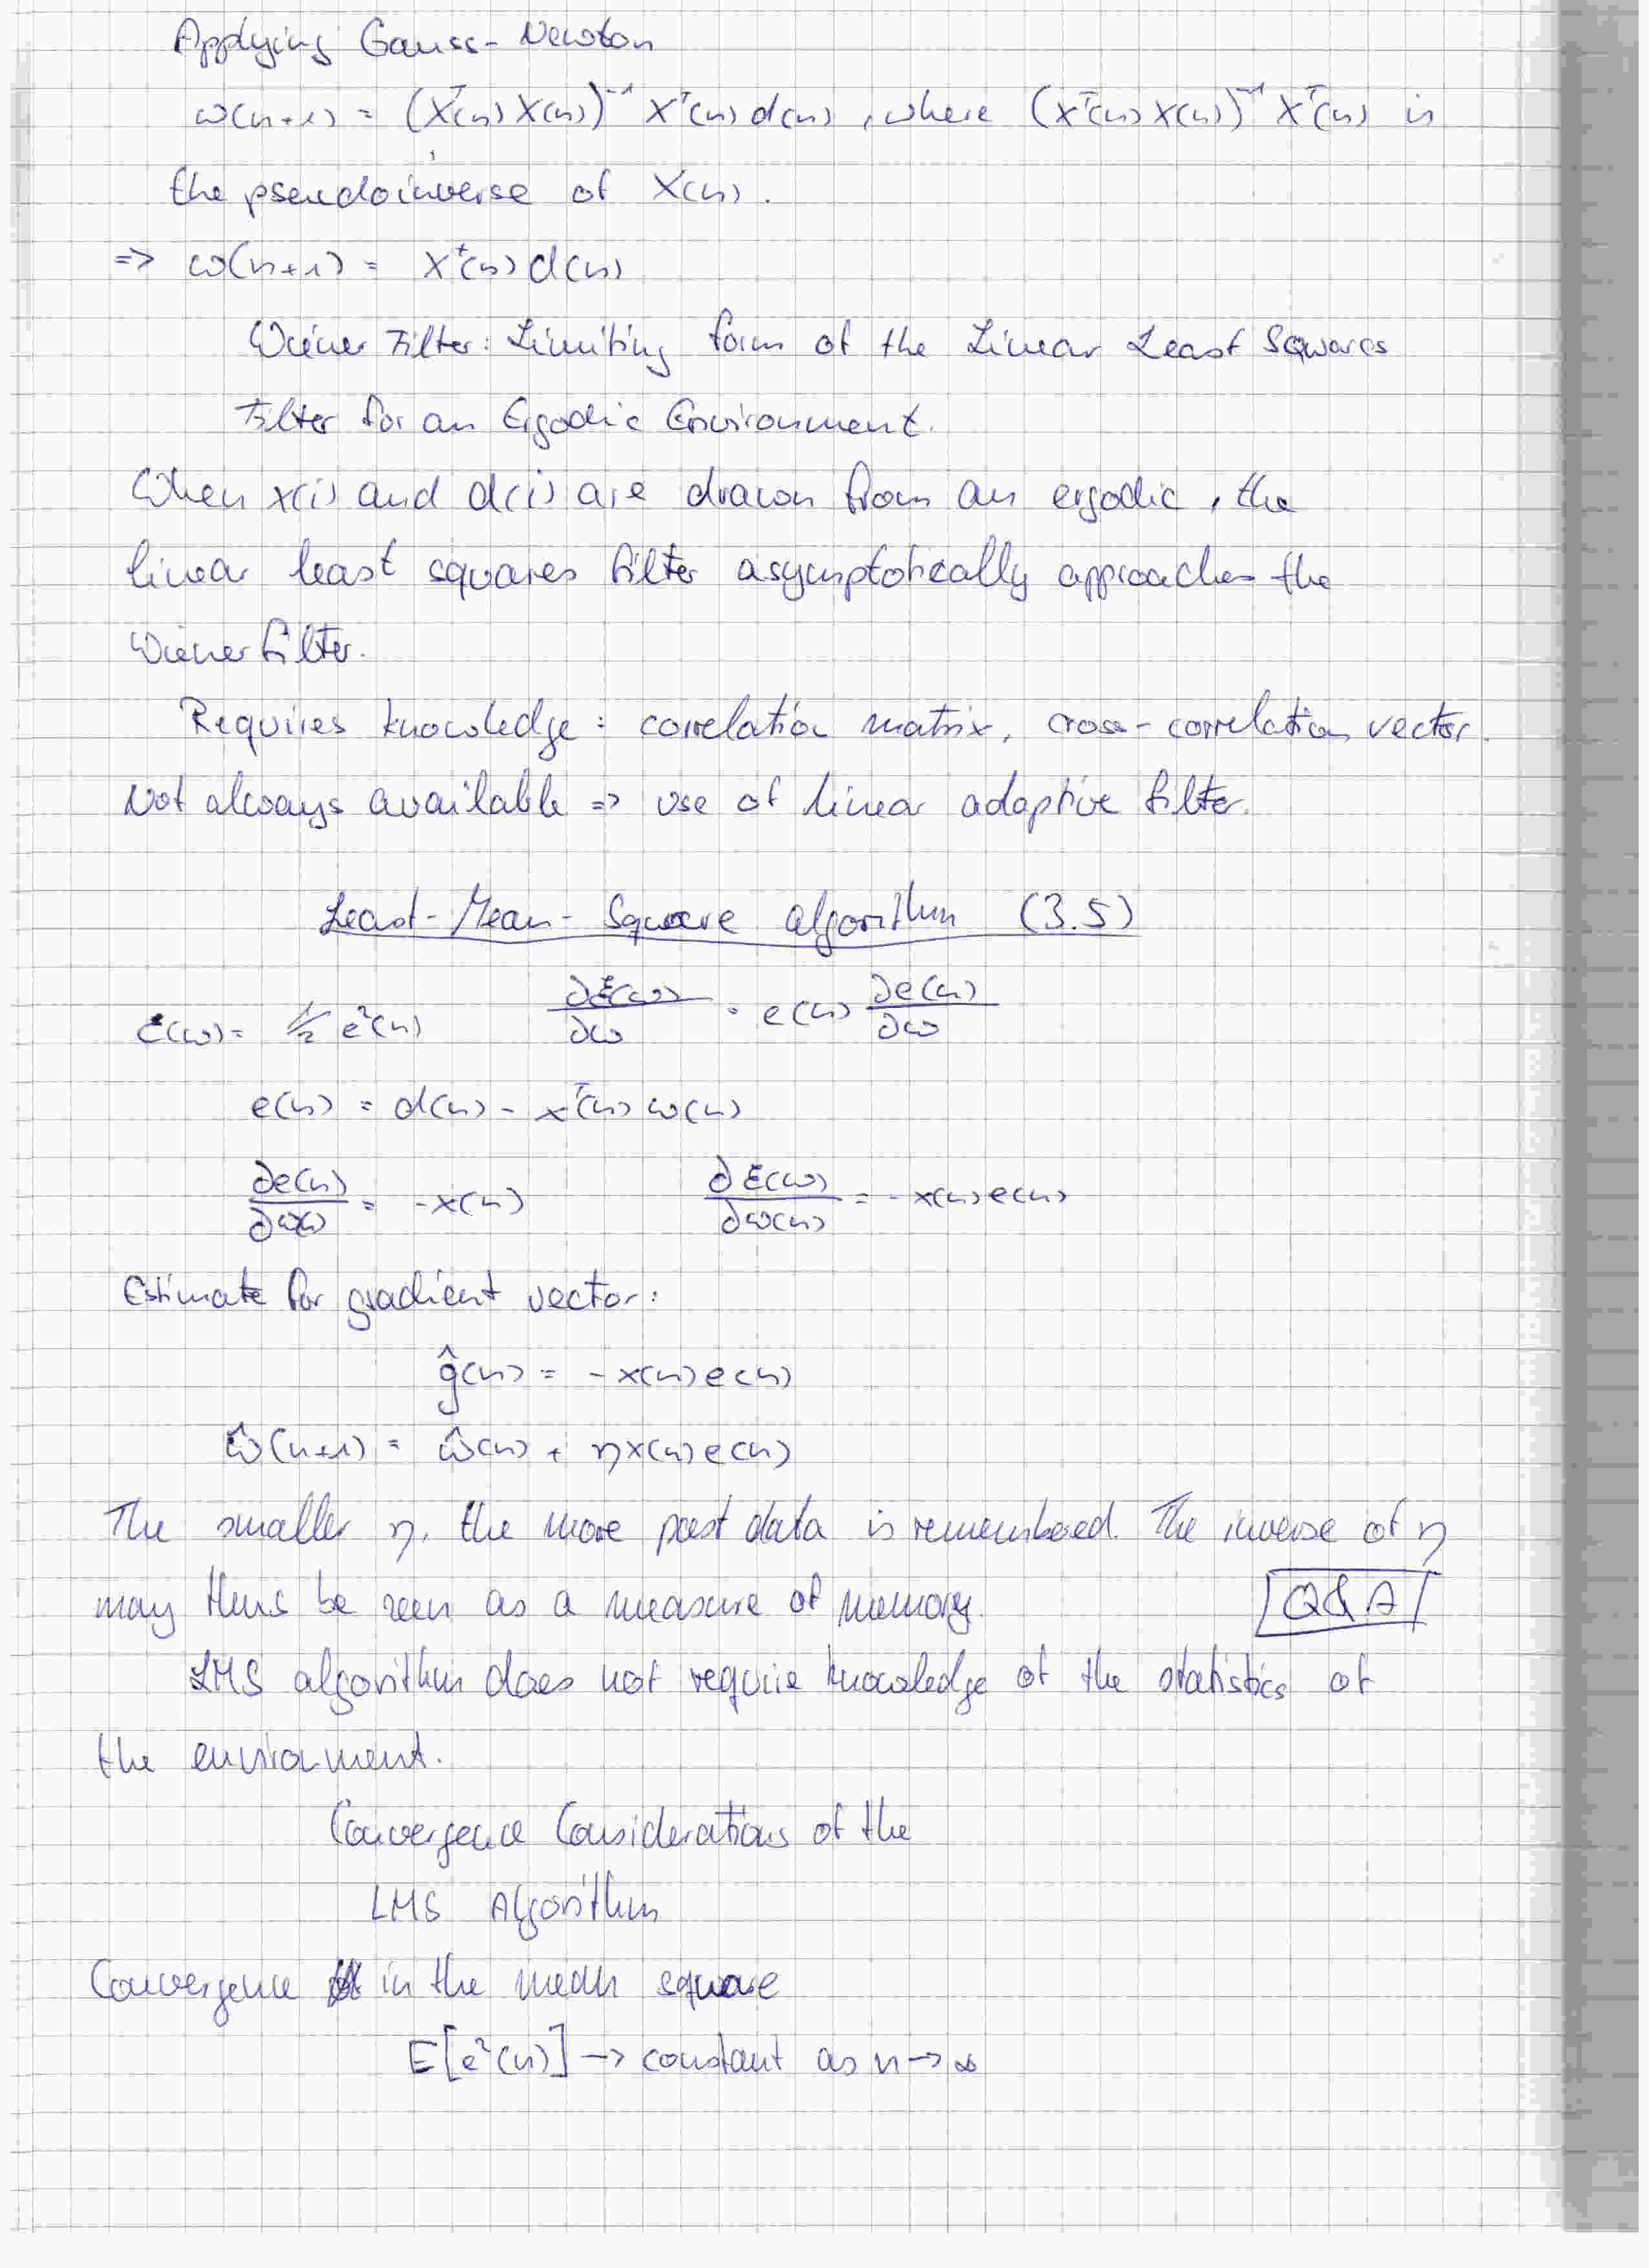
\includegraphics[width=0.7\textheight]{08.jpg}
	\caption{summary 5}
	\label{fig5}
\end{figure}

\begin{figure}[ht]
	\centering
  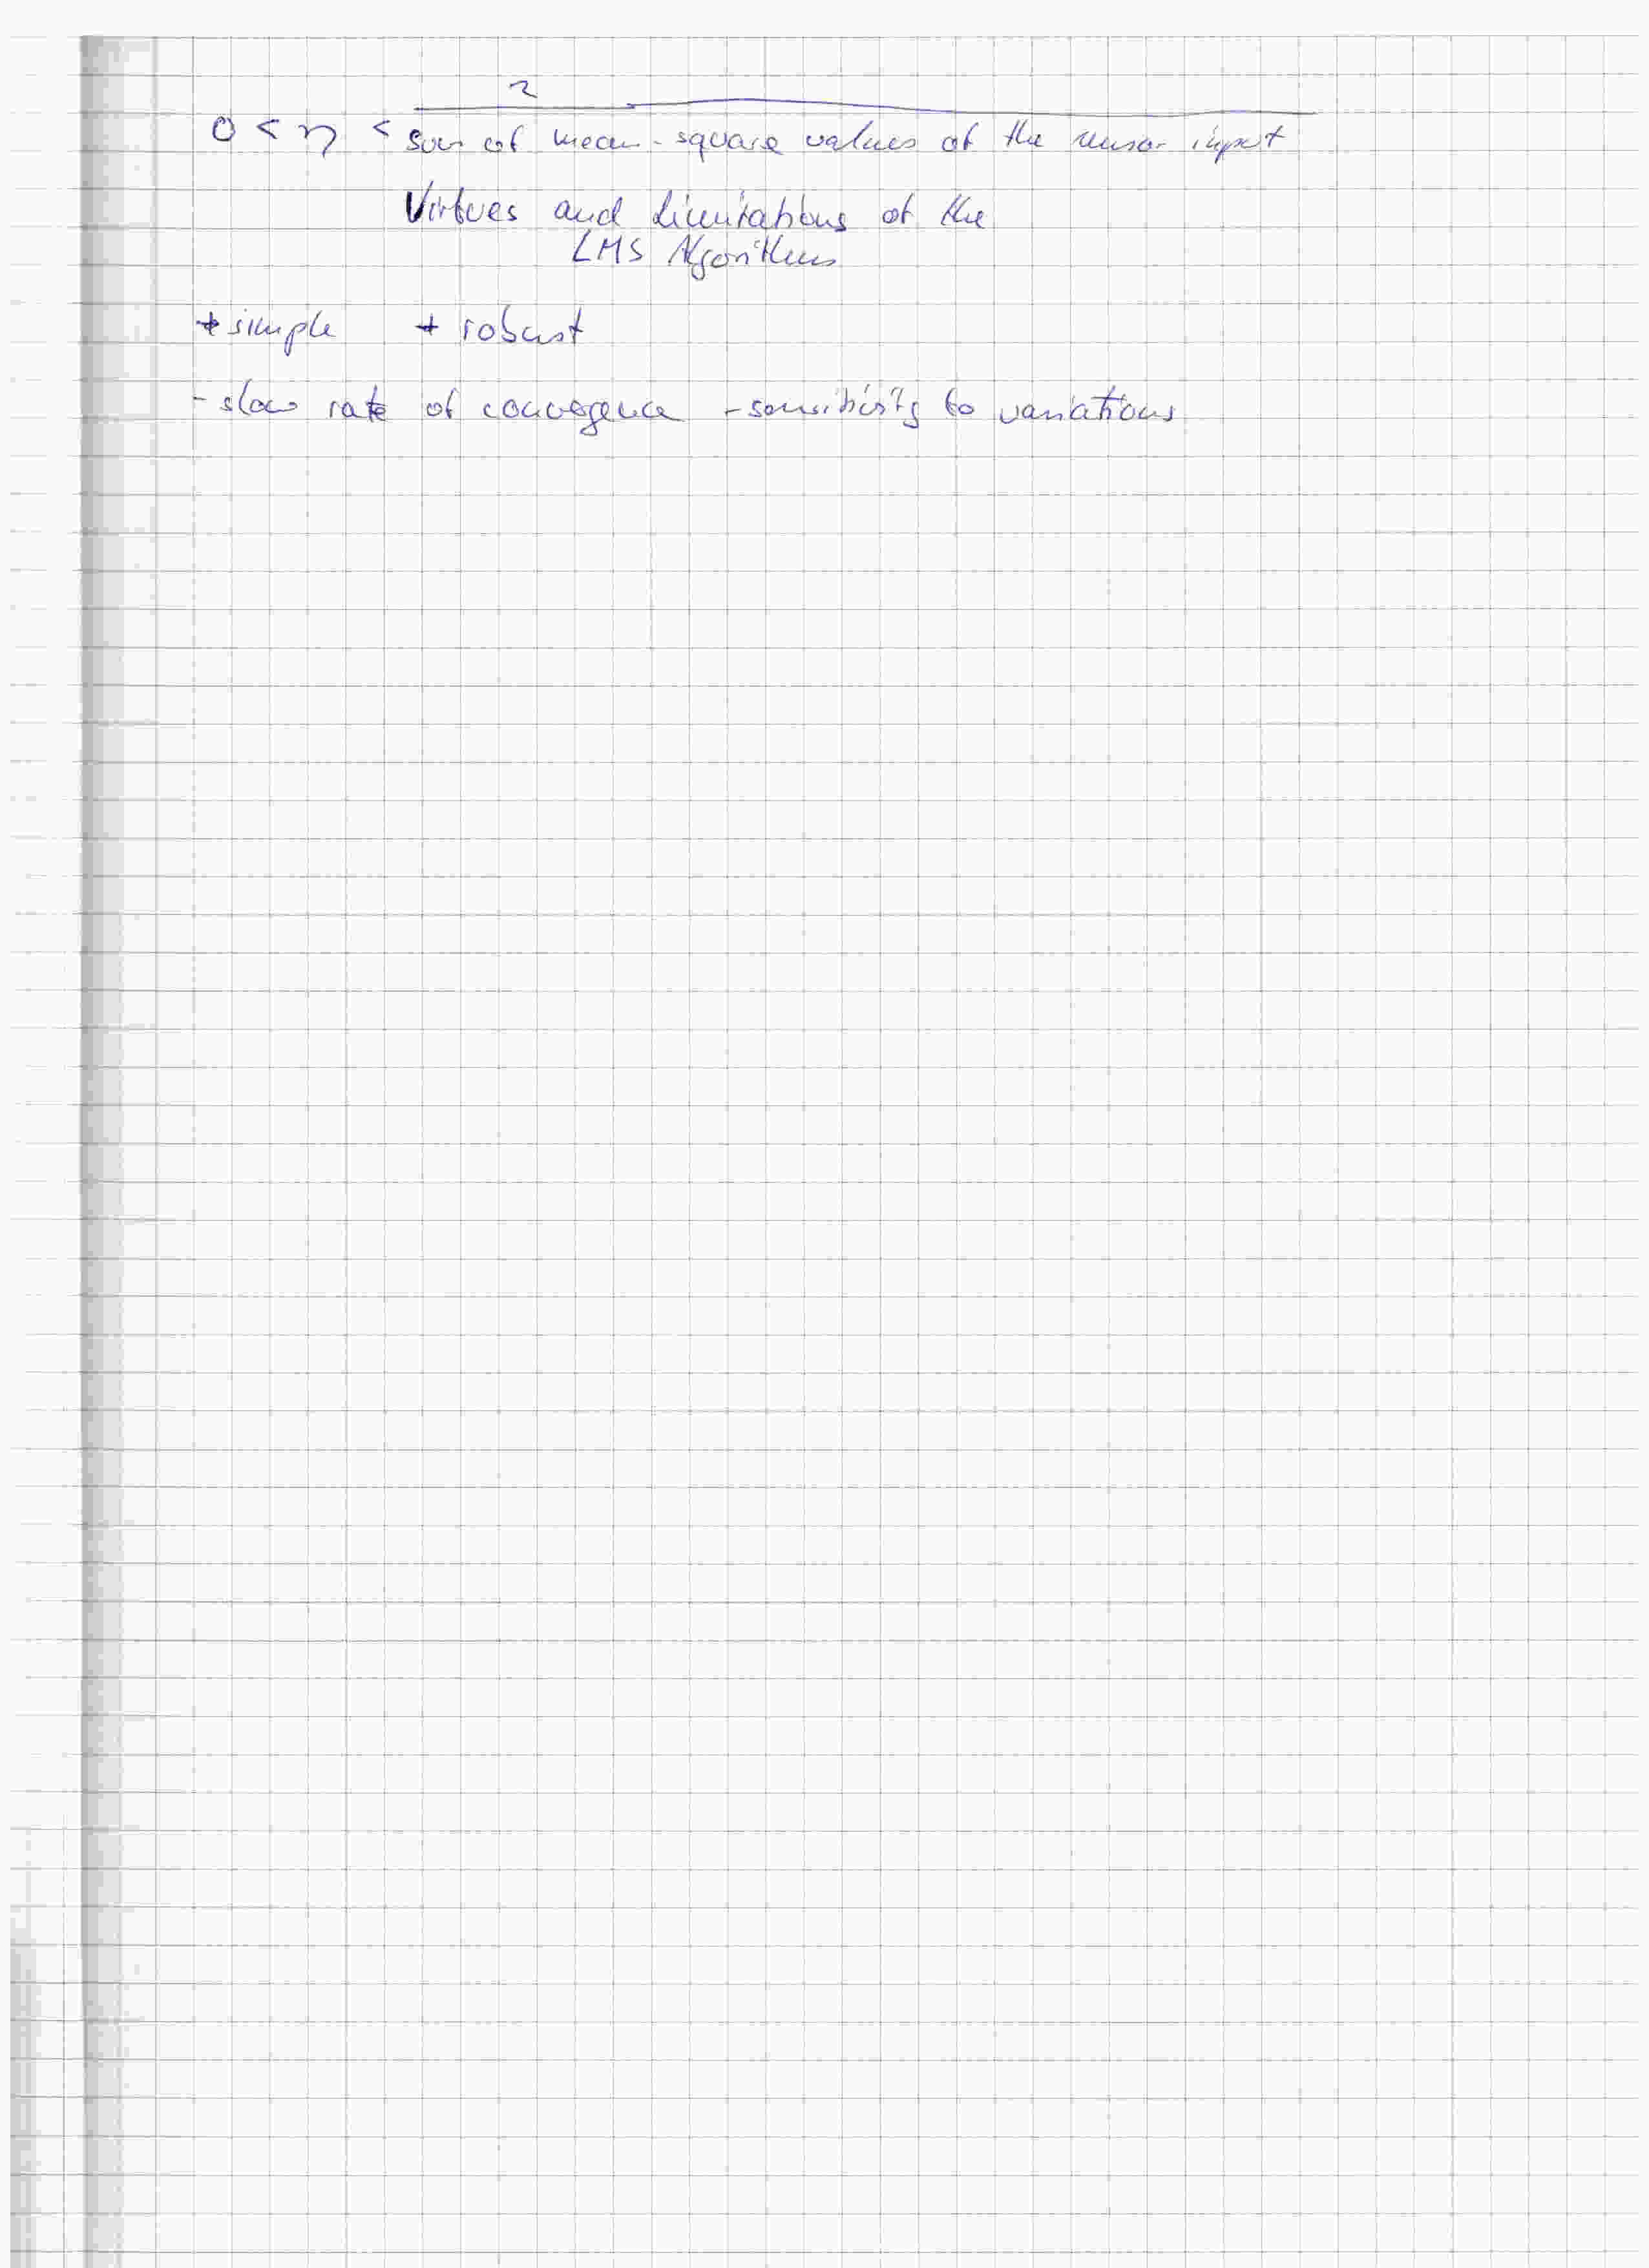
\includegraphics[width=0.7\textheight]{09.jpg}
	\caption{summary 6}
	\label{fig6}
\end{figure}



\section{Ex3.1}

See figure \ref{fig3_1}
\begin{figure}[ht]
	\centering
  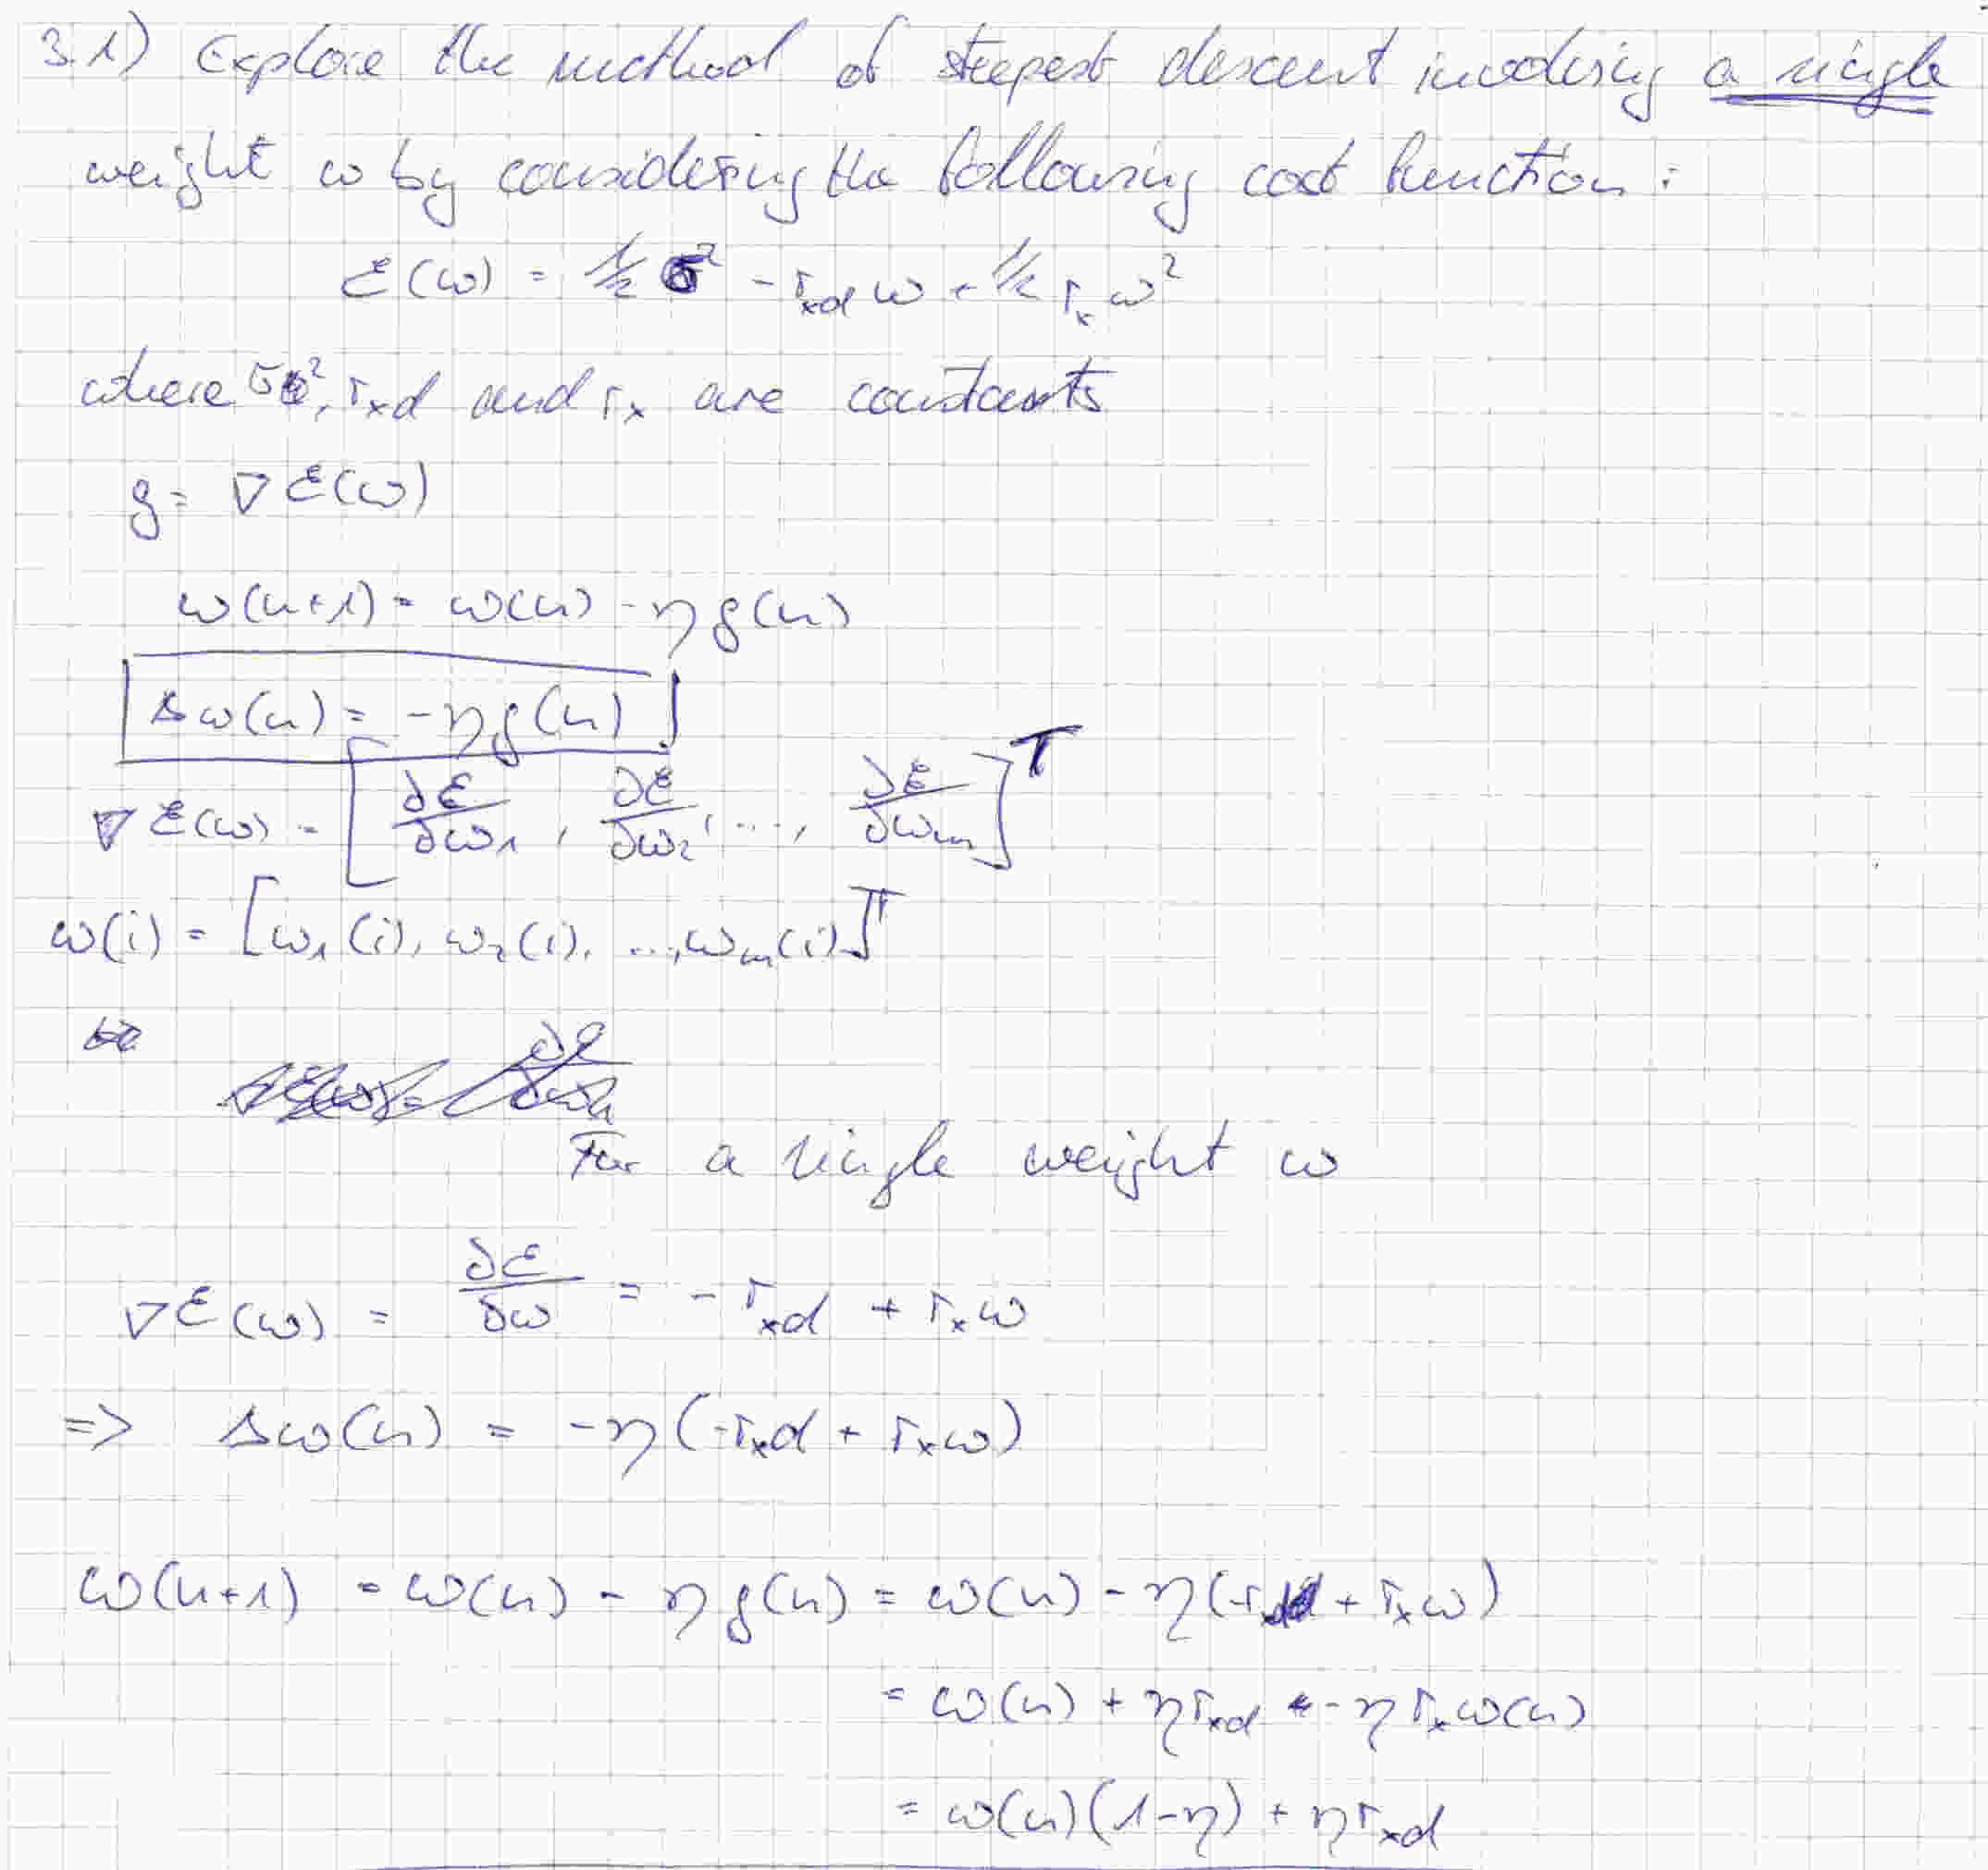
\includegraphics[width=0.7\textheight]{ex3_1.jpg}
	\caption{ex3.1}
	\label{fig3_1}
\end{figure}


\section{Ex3.2}
\subsection{a}
See figure \ref{fig3_2a}
\begin{figure}[ht]
	\centering
  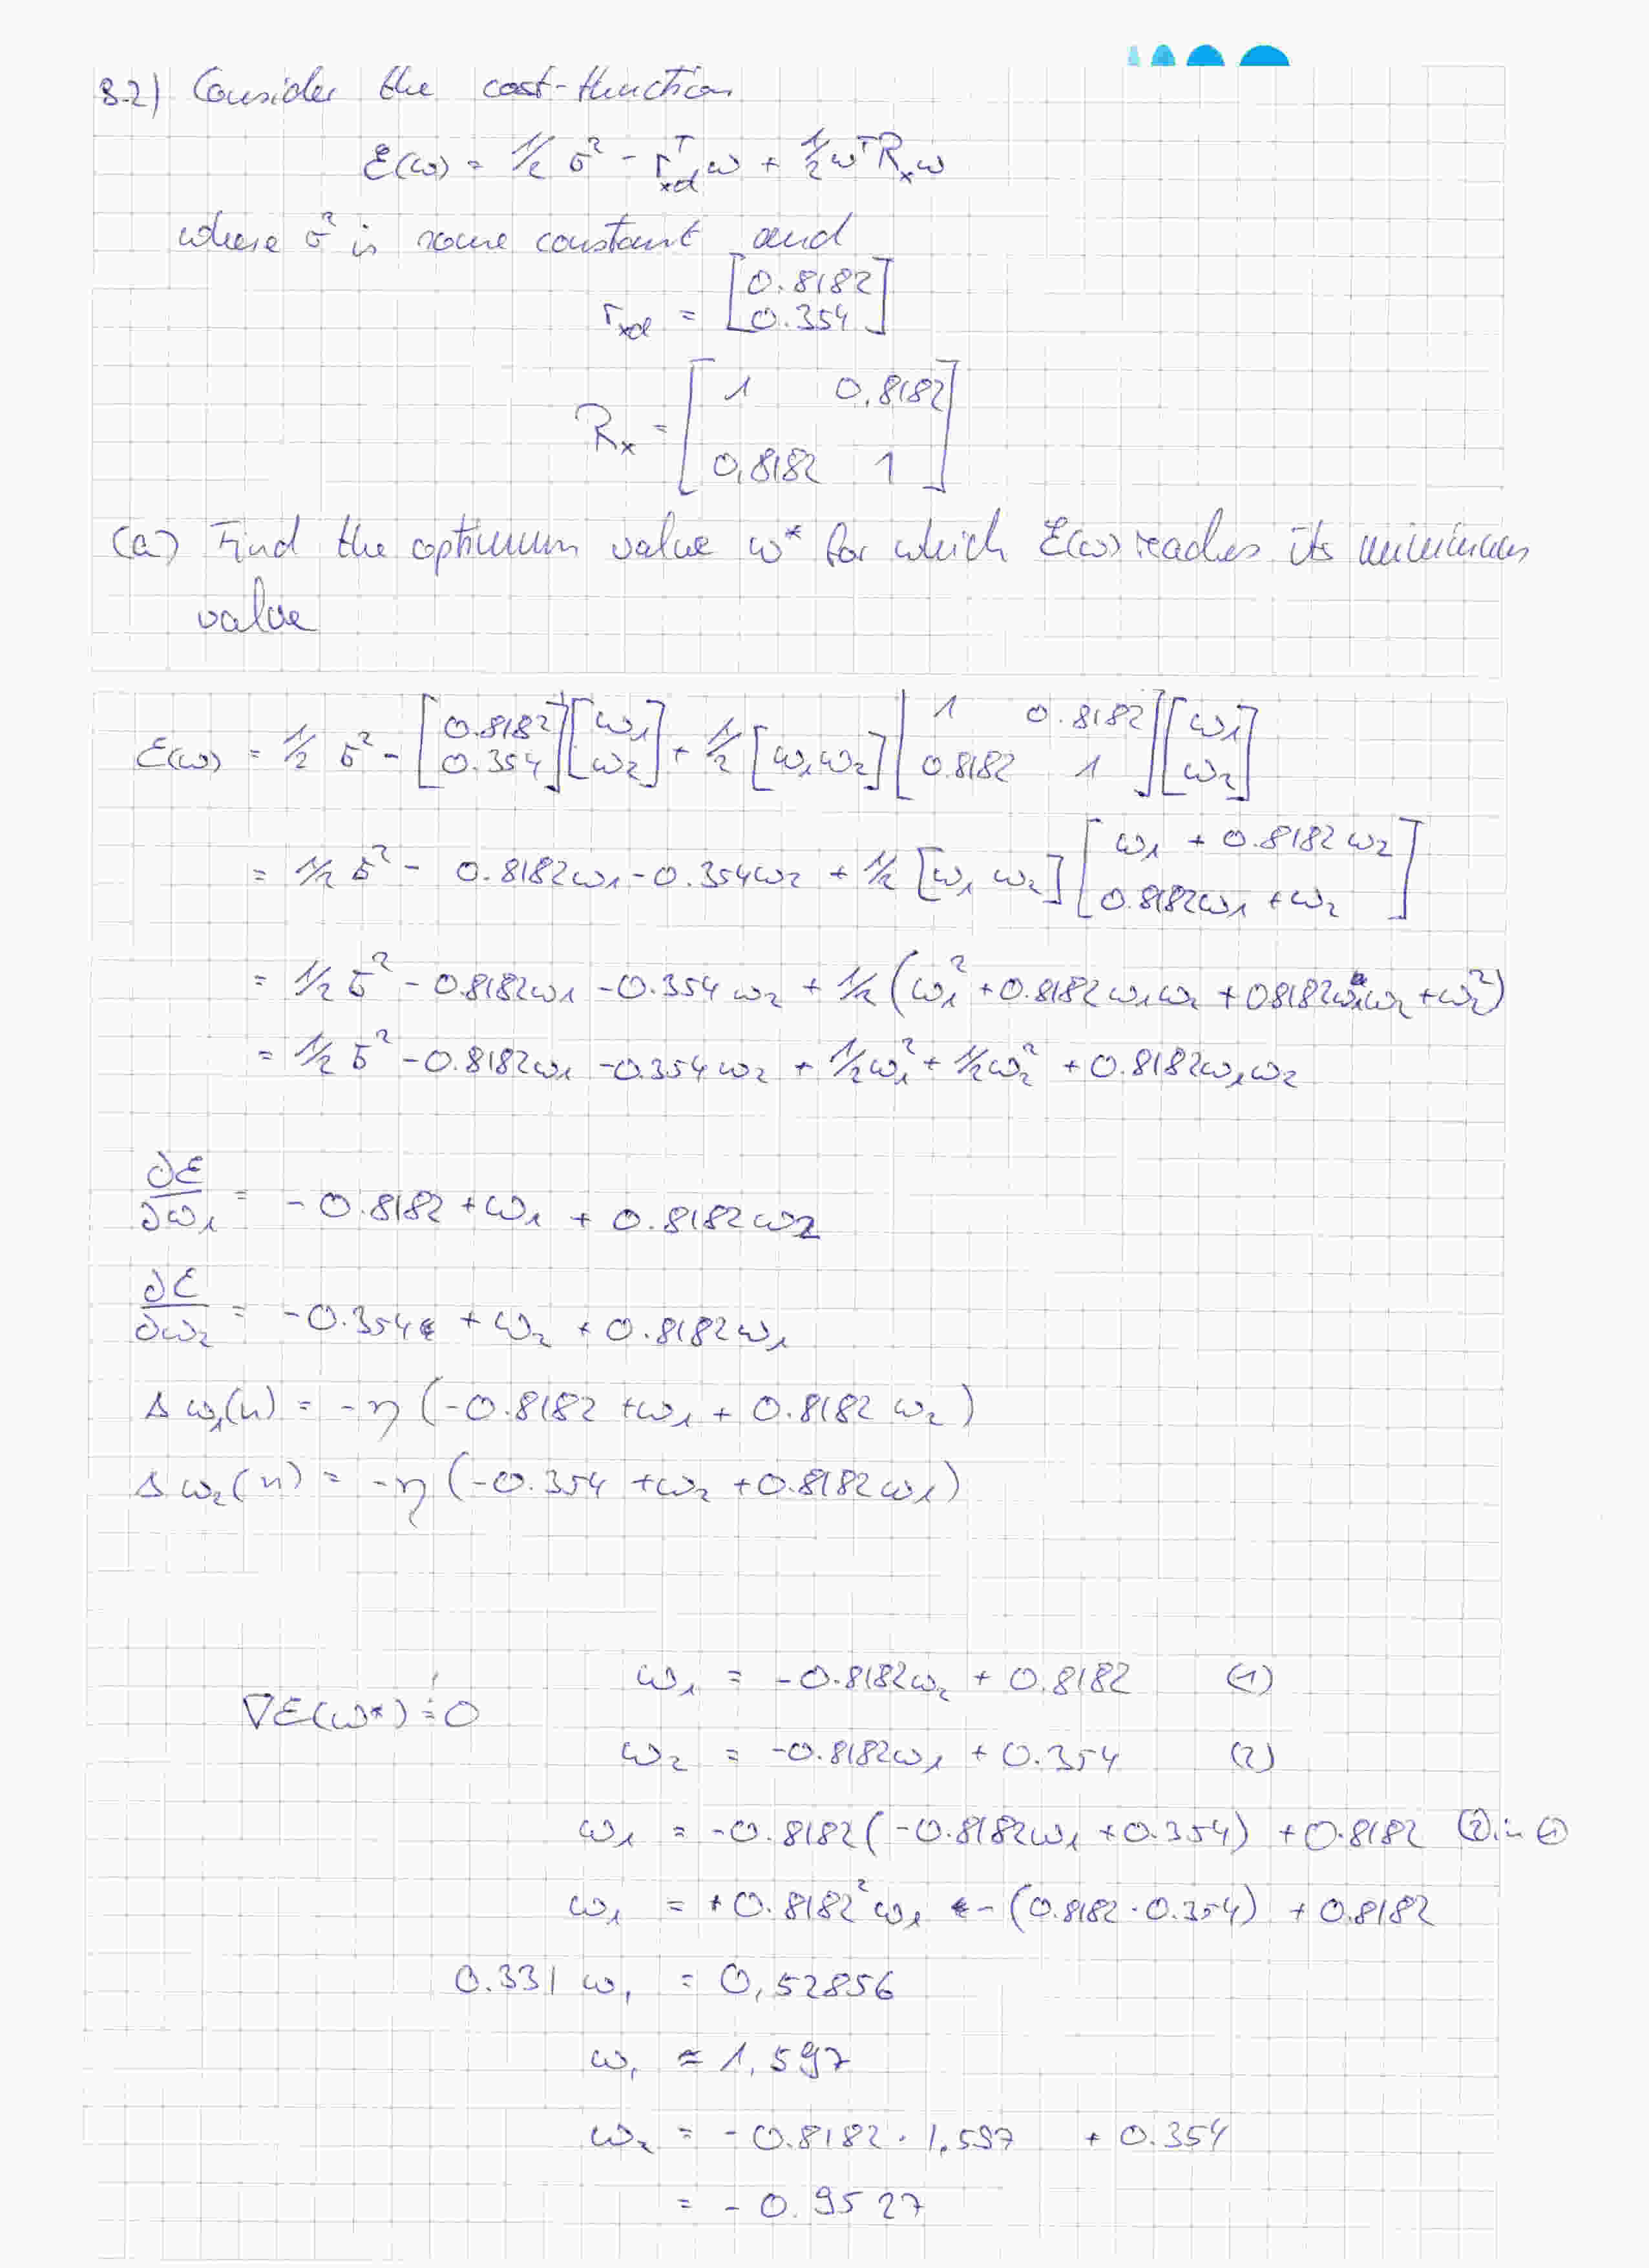
\includegraphics[width=0.7\textheight]{ex3_2a.jpg}
	\caption{ex3.2a}
	\label{fig3_2a}
\end{figure}

\subsection{b}
See figure \ref{fig3_2b} for formulas.
\begin{figure}[ht]
	\centering
  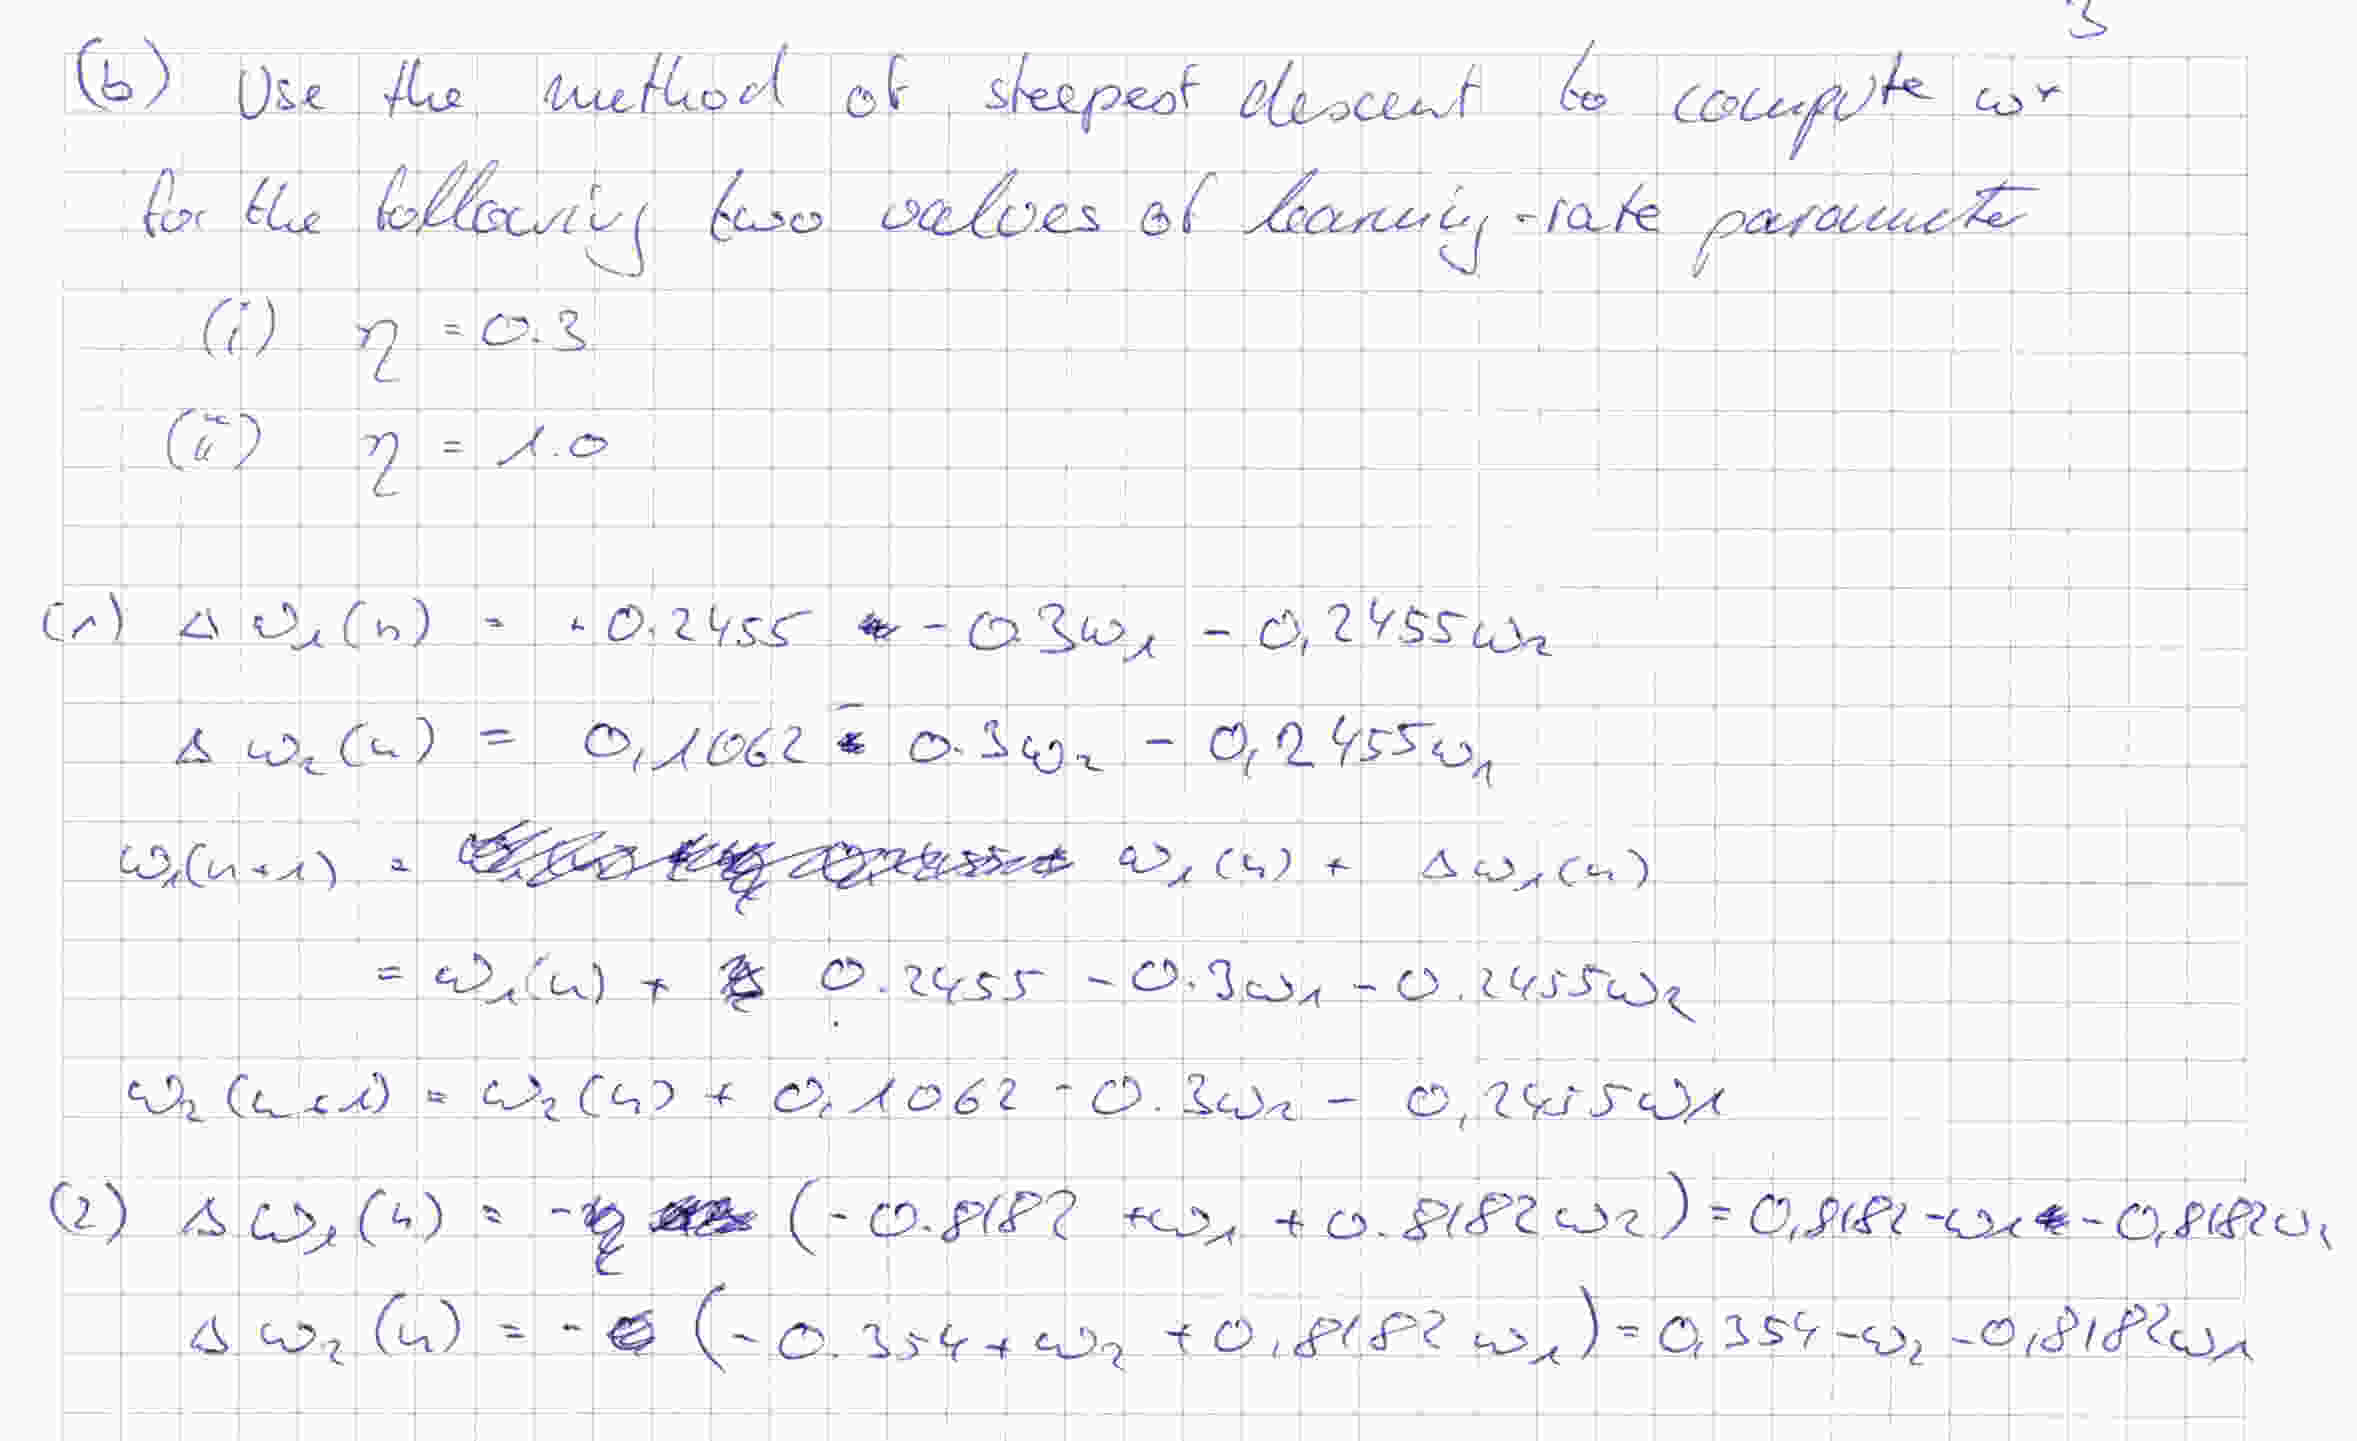
\includegraphics[width=0.7\textheight]{ex3_2b.jpg}
	\caption{ex3.2b}
	\label{fig3_2b}
\end{figure}


\end{document}